
%% bare_conf.tex
%% V1.3
%% 2007/01/11
%% by Michael Shell
%% See:
%% http://www.michaelshell.org/
%% for current contact information.
%%
%% This is a skeleton file demonstrating the use of IEEEtran.cls
%% (requires IEEEtran.cls version 1.7 or later) with an IEEE conference paper.
%%
%% Support sites:
%% http://www.michaelshell.org/tex/ieeetran/
%% http://www.ctan.org/tex-archive/macros/latex/contrib/IEEEtran/
%% and
%% http://www.ieee.org/

%%*************************************************************************
%% Legal Notice:
%% This code is offered as-is without any warranty either expressed or
%% implied; without even the implied warranty of MERCHANTABILITY or
%% FITNESS FOR A PARTICULAR PURPOSE! 
%% User assumes all risk.
%% In no event shall IEEE or any contributor to this code be liable for
%% any damages or losses, including, but not limited to, incidental,
%% consequential, or any other damages, resulting from the use or misuse
%% of any information contained here.
%%
%% All comments are the opinions of their respective authors and are not
%% necessarily endorsed by the IEEE.
%%
%% This work is distributed under the LaTeX Project Public License (LPPL)
%% ( http://www.latex-project.org/ ) version 1.3, and may be freely used,
%% distributed and modified. A copy of the LPPL, version 1.3, is included
%% in the base LaTeX documentation of all distributions of LaTeX released
%% 2003/12/01 or later.
%% Retain all contribution notices and credits.
%% ** Modified files should be clearly indicated as such, including  **
%% ** renaming them and changing author support contact information. **
%%
%% File list of work: IEEEtran.cls, IEEEtran_HOWTO.pdf, bare_adv.tex,
%%                    bare_conf.tex, bare_jrnl.tex, bare_jrnl_compsoc.tex
%%*************************************************************************

% *** Authors should verify (and, if needed, correct) their LaTeX system  ***
% *** with the testflow diagnostic prior to trusting their LaTeX platform ***
% *** with production work. IEEE's font choices can trigger bugs that do  ***
% *** not appear when using other class files.                            ***
% The testflow support page is at:
% http://www.michaelshell.org/tex/testflow/



% Note that the a4paper option is mainly intended so that authors in
% countries using A4 can easily print to A4 and see how their papers will
% look in print - the typesetting of the document will not typically be
% affected with changes in paper size (but the bottom and side margins will).
% Use the testflow package mentioned above to verify correct handling of
% both paper sizes by the user's LaTeX system.
%
% Also note that the "draftcls" or "draftclsnofoot", not "draft", option
% should be used if it is desired that the figures are to be displayed in
% draft mode.
%
\documentclass[conference]{IEEEtran}
% Add the compsoc option for Computer Society conferences.
%
% If IEEEtran.cls has not been installed into the LaTeX system files,
% manually specify the path to it like:
% \documentclass[conference]{../sty/IEEEtran}





% Some very useful LaTeX packages include:
% (uncomment the ones you want to load)


% *** MISC UTILITY PACKAGES ***
%
%\usepackage{ifpdf}
% Heiko Oberdiek's ifpdf.sty is very useful if you need conditional
% compilation based on whether the output is pdf or dvi.
% usage:
% \ifpdf
%   % pdf code
% \else
%   % dvi code
% \fi
% The latest version of ifpdf.sty can be obtained from:
% http://www.ctan.org/tex-archive/macros/latex/contrib/oberdiek/
% Also, note that IEEEtran.cls V1.7 and later provides a builtin
% \ifCLASSINFOpdf conditional that works the same way.
% When switching from latex to pdflatex and vice-versa, the compiler may
% have to be run twice to clear warning/error messages.






% *** CITATION PACKAGES ***
%
%\usepackage{cite}
% cite.sty was written by Donald Arseneau
% V1.6 and later of IEEEtran pre-defines the format of the cite.sty package
% \cite{} output to follow that of IEEE. Loading the cite package will
% result in citation numbers being automatically sorted and properly
% "compressed/ranged". e.g., [1], [9], [2], [7], [5], [6] without using
% cite.sty will become [1], [2], [5]--[7], [9] using cite.sty. cite.sty's
% \cite will automatically add leading space, if needed. Use cite.sty's
% noadjust option (cite.sty V3.8 and later) if you want to turn this off.
% cite.sty is already installed on most LaTeX systems. Be sure and use
% version 4.0 (2003-05-27) and later if using hyperref.sty. cite.sty does
% not currently provide for hyperlinked citations.
% The latest version can be obtained at:
% http://www.ctan.org/tex-archive/macros/latex/contrib/cite/
% The documentation is contained in the cite.sty file itself.






% *** GRAPHICS RELATED PACKAGES ***
%
% \ifCLASSINFOpdf
  \usepackage[pdftex]{graphicx}
  % declare the path(s) where your graphic files are
  \graphicspath{{../figures/}}
  % and their extensions so you won't have to specify these with
  % every instance of \includegraphics
  \DeclareGraphicsExtensions{.pdf,.jpeg,.png}
% \else
  % or other class option (dvipsone, dvipdf, if not using dvips). graphicx
  % will default to the driver specified in the system graphics.cfg if no
  % driver is specified.
  % \usepackage[dvips]{graphicx}
  % declare the path(s) where your graphic files are
  % \graphicspath{{../eps/}}
  % and their extensions so you won't have to specify these with
  % every instance of \includegraphics
  % \DeclareGraphicsExtensions{.eps}
% \fi
% graphicx was written by David Carlisle and Sebastian Rahtz. It is
% required if you want graphics, photos, etc. graphicx.sty is already
% installed on most LaTeX systems. The latest version and documentation can
% be obtained at: 
% http://www.ctan.org/tex-archive/macros/latex/required/graphics/
% Another good source of documentation is "Using Imported Graphics in
% LaTeX2e" by Keith Reckdahl which can be found as epslatex.ps or
% epslatex.pdf at: http://www.ctan.org/tex-archive/info/
%
% latex, and pdflatex in dvi mode, support graphics in encapsulated
% postscript (.eps) format. pdflatex in pdf mode supports graphics
% in .pdf, .jpeg, .png and .mps (metapost) formats. Users should ensure
% that all non-photo figures use a vector format (.eps, .pdf, .mps) and
% not a bitmapped formats (.jpeg, .png). IEEE frowns on bitmapped formats
% which can result in "jaggedy"/blurry rendering of lines and letters as
% well as large increases in file sizes.
%
% You can find documentation about the pdfTeX application at:
% http://www.tug.org/applications/pdftex





% *** MATH PACKAGES ***
%
\usepackage[cmex10]{amsmath}
% A popular package from the American Mathematical Society that provides
% many useful and powerful commands for dealing with mathematics. If using
% it, be sure to load this package with the cmex10 option to ensure that
% only type 1 fonts will utilized at all point sizes. Without this option,
% it is possible that some math symbols, particularly those within
% footnotes, will be rendered in bitmap form which will result in a
% document that can not be IEEE Xplore compliant!
%
% Also, note that the amsmath package sets \interdisplaylinepenalty to 10000
% thus preventing page breaks from occurring within multiline equations. Use:
%\interdisplaylinepenalty=2500
% after loading amsmath to restore such page breaks as IEEEtran.cls normally
% does. amsmath.sty is already installed on most LaTeX systems. The latest
% version and documentation can be obtained at:
% http://www.ctan.org/tex-archive/macros/latex/required/amslatex/math/





% *** SPECIALIZED LIST PACKAGES ***
%
%\usepackage{algorithmic}
% algorithmic.sty was written by Peter Williams and Rogerio Brito.
% This package provides an algorithmic environment fo describing algorithms.
% You can use the algorithmic environment in-text or within a figure
% environment to provide for a floating algorithm. Do NOT use the algorithm
% floating environment provided by algorithm.sty (by the same authors) or
% algorithm2e.sty (by Christophe Fiorio) as IEEE does not use dedicated
% algorithm float types and packages that provide these will not provide
% correct IEEE style captions. The latest version and documentation of
% algorithmic.sty can be obtained at:
% http://www.ctan.org/tex-archive/macros/latex/contrib/algorithms/
% There is also a support site at:
% http://algorithms.berlios.de/index.html
% Also of interest may be the (relatively newer and more customizable)
% algorithmicx.sty package by Szasz Janos:
% http://www.ctan.org/tex-archive/macros/latex/contrib/algorithmicx/




% *** ALIGNMENT PACKAGES ***
%
%\usepackage{array}
% Frank Mittelbach's and David Carlisle's array.sty patches and improves
% the standard LaTeX2e array and tabular environments to provide better
% appearance and additional user controls. As the default LaTeX2e table
% generation code is lacking to the point of almost being broken with
% respect to the quality of the end results, all users are strongly
% advised to use an enhanced (at the very least that provided by array.sty)
% set of table tools. array.sty is already installed on most systems. The
% latest version and documentation can be obtained at:
% http://www.ctan.org/tex-archive/macros/latex/required/tools/


%\usepackage{mdwmath}
%\usepackage{mdwtab}
% Also highly recommended is Mark Wooding's extremely powerful MDW tools,
% especially mdwmath.sty and mdwtab.sty which are used to format equations
% and tables, respectively. The MDWtools set is already installed on most
% LaTeX systems. The lastest version and documentation is available at:
% http://www.ctan.org/tex-archive/macros/latex/contrib/mdwtools/


% IEEEtran contains the IEEEeqnarray family of commands that can be used to
% generate multiline equations as well as matrices, tables, etc., of high
% quality.


%\usepackage{eqparbox}
% Also of notable interest is Scott Pakin's eqparbox package for creating
% (automatically sized) equal width boxes - aka "natural width parboxes".
% Available at:
% http://www.ctan.org/tex-archive/macros/latex/contrib/eqparbox/





% *** SUBFIGURE PACKAGES ***
%\usepackage[tight,footnotesize]{subfigure}
% subfigure.sty was written by Steven Douglas Cochran. This package makes it
% easy to put subfigures in your figures. e.g., "Figure 1a and 1b". For IEEE
% work, it is a good idea to load it with the tight package option to reduce
% the amount of white space around the subfigures. subfigure.sty is already
% installed on most LaTeX systems. The latest version and documentation can
% be obtained at:
% http://www.ctan.org/tex-archive/obsolete/macros/latex/contrib/subfigure/
% subfigure.sty has been superceeded by subfig.sty.



%\usepackage[caption=false]{caption}
%\usepackage[font=footnotesize]{subfig}
% subfig.sty, also written by Steven Douglas Cochran, is the modern
% replacement for subfigure.sty. However, subfig.sty requires and
% automatically loads Axel Sommerfeldt's caption.sty which will override
% IEEEtran.cls handling of captions and this will result in nonIEEE style
% figure/table captions. To prevent this problem, be sure and preload
% caption.sty with its "caption=false" package option. This is will preserve
% IEEEtran.cls handing of captions. Version 1.3 (2005/06/28) and later 
% (recommended due to many improvements over 1.2) of subfig.sty supports
% the caption=false option directly:
%\usepackage[caption=false,font=footnotesize]{subfig}
%
% The latest version and documentation can be obtained at:
% http://www.ctan.org/tex-archive/macros/latex/contrib/subfig/
% The latest version and documentation of caption.sty can be obtained at:
% http://www.ctan.org/tex-archive/macros/latex/contrib/caption/




% *** FLOAT PACKAGES ***
%
%\usepackage{fixltx2e}
% fixltx2e, the successor to the earlier fix2col.sty, was written by
% Frank Mittelbach and David Carlisle. This package corrects a few problems
% in the LaTeX2e kernel, the most notable of which is that in current
% LaTeX2e releases, the ordering of single and double column floats is not
% guaranteed to be preserved. Thus, an unpatched LaTeX2e can allow a
% single column figure to be placed prior to an earlier double column
% figure. The latest version and documentation can be found at:
% http://www.ctan.org/tex-archive/macros/latex/base/


\usepackage{flafter}
%\usepackage{stfloats}
% stfloats.sty was written by Sigitas Tolusis. This package gives LaTeX2e
% the ability to do double column floats at the bottom of the page as well
% as the top. (e.g., "\begin{figure*}[!b]" is not normally possible in
% LaTeX2e). It also provides a command:
%\fnbelowfloat
% to enable the placement of footnotes below bottom floats (the standard
% LaTeX2e kernel puts them above bottom floats). This is an invasive package
% which rewrites many portions of the LaTeX2e float routines. It may not work
% with other packages that modify the LaTeX2e float routines. The latest
% version and documentation can be obtained at:
% http://www.ctan.org/tex-archive/macros/latex/contrib/sttools/
% Documentation is contained in the stfloats.sty comments as well as in the
% presfull.pdf file. Do not use the stfloats baselinefloat ability as IEEE
% does not allow \baselineskip to stretch. Authors submitting work to the
% IEEE should note that IEEE rarely uses double column equations and
% that authors should try to avoid such use. Do not be tempted to use the
% cuted.sty or midfloat.sty packages (also by Sigitas Tolusis) as IEEE does
% not format its papers in such ways.





% *** PDF, URL AND HYPERLINK PACKAGES ***
%
\usepackage{url}
% url.sty was written by Donald Arseneau. It provides better support for
% handling and breaking URLs. url.sty is already installed on most LaTeX
% systems. The latest version can be obtained at:
% http://www.ctan.org/tex-archive/macros/latex/contrib/misc/
% Read the url.sty source comments for usage information. Basically,
% \url{my_url_here}.





% *** Do not adjust lengths that control margins, column widths, etc. ***
% *** Do not use packages that alter fonts (such as pslatex).         ***
% There should be no need to do such things with IEEEtran.cls V1.6 and later.
% (Unless specifically asked to do so by the journal or conference you plan
% to submit to, of course. )

\let\olditemize\itemize
\def\itemize{\olditemize\itemsep=0pt }

% correct bad hyphenation here
\hyphenation{eli-mi-na-tion ope-ra-tor ope-ra-tors appli-ca-tion sto-ra-ges Hor-rocks re-fe-ren-ces}

\renewenvironment{description}[1][57pt]
   {\list{}{\labelwidth=1.5cm \leftmargin=#1 \setlength{\itemsep}{0pt}
   \let\makelabel\descriptionlabel}}
   {\endlist}

\begin{document}
%
% paper title
% can use linebreaks \\ within to get better formatting as desired
\title{Low size FFT core for OFDM communications}


% author names and affiliations
% use a multiple column layout for up to three different
% affiliations
% \author{
% \IEEEauthorblockN{XXXXXX XXXXXXXXX, XXXXXXXX X. XXXXXXXXX\\ and XXXXXXX XXXXXX}
% \IEEEauthorblockA{XXXXXXXXXXX XX XXXXXX XXXXX,\\
% XXXXXXXX XX XXXXXXXXXX,\\
% XXXXXXXXXXX XX XXXXXXXX XXXXXXXXX,\\
% XXXXXX XXXXX, XXXXXXXXX\\
% \{XXXXXXXXXX,XXXXXXXXXX,XXXXXXX\}@XX.XXX.XX}
% \and
% \IEEEauthorblockN{XXXXX XXXXXXXXX}
% \IEEEauthorblockA{XXXXXXXXXXX XX XXXXXX XXXXX,\\
% XXXXXXXX XX XXXXXXXXXX,\\
% XXXXXXXXXXX XX XXXXXXXX XXXXXXXXX\\
% XXX XXXXXXXXXXXXXXX,\\
% XXXXXX XXXXX, XXXXXXXXX\\
% XXX@XX.XXX.XX}
% }

\author{
\IEEEauthorblockN{Andr\'es D. Cassagnes, Federico G. Zacchigna and Octavio Alpago}
\IEEEauthorblockA{Universidad de Buenos Aires,\\
Facultad de Ingenier\'ia,\\
Laboratorio de Sistemas Embebidos,\\
Buenos Aires, Argentina\\
\{acassagnes,fzacchigna,oalpago\}@fi.uba.ar}
\and
\IEEEauthorblockN{Ariel Lutenberg}
\IEEEauthorblockA{Universidad de Buenos Aires,\\
Facultad de Ingenier\'ia,\\
Laboratorio de Sistemas Embebidos\\
and CONICET-GICSAFe,\\
Buenos Aires, Argentina\\
lse@fi.uba.ar}
}


% \author{\IEEEauthorblockN{Michael Shell}
% \IEEEauthorblockA{School of Electrical and\\Computer Engineering\\
% Georgia Institute of Technology\\
% Atlanta, Georgia 30332--0250\\
% Email: http://www.michaelshell.org/contact.html}
% \and
% \IEEEauthorblockN{Homer Simpson}
% \IEEEauthorblockA{Twentieth Century Fox\\
% Springfield, USA\\
% Email: homer@thesimpsons.com}
% \and
% \IEEEauthorblockN{Octavio H. Alpago and Federico G. Zacchigna}
% \IEEEauthorblockA{Starfleet Academy\\
% San Francisco, California 96678-2391\\
% Telephone: (800) 555--1212\\
% Fax: (888) 555--1212}}

% conference papers do not typically use \thanks and this command
% is locked out in conference mode. If really needed, such as for
% the acknowledgment of grants, issue a \IEEEoverridecommandlockouts
% after \documentclass

% for over three affiliations, or if they all won't fit within the width
% of the page, use this alternative format:
%
%\author{\IEEEauthorblockN{Michael Shell\IEEEauthorrefmark{1},
%Homer Simpson\IEEEauthorrefmark{2},
%James Kirk\IEEEauthorrefmark{3}, 
%Montgomery Scott\IEEEauthorrefmark{3} and
%Eldon Tyrell\IEEEauthorrefmark{4}}
%\IEEEauthorblockA{\IEEEauthorrefmark{1}School of Electrical and Computer Engineering\\
%Georgia Institute of Technology,
%Atlanta, Georgia 30332--0250\\ Email: see http://www.michaelshell.org/contact.html}
%\IEEEauthorblockA{\IEEEauthorrefmark{2}Twentieth Century Fox, Springfield, USA\\
%Email: homer@thesimpsons.com}
%\IEEEauthorblockA{\IEEEauthorrefmark{3}Starfleet Academy, San Francisco, California 96678-2391\\
%Telephone: (800) 555--1212, Fax: (888) 555--1212}
%\IEEEauthorblockA{\IEEEauthorrefmark{4}Tyrell Inc., 123 Replicant Street, Los Angeles, California 90210--4321}}




% use for special paper notices
%\IEEEspecialpapernotice{(Invited Paper)}




% make the title area
\maketitle


\begin{abstract}
%\boldmath
In this work two FFT architectures to be used in a ISDB-T OFDM modulator are presented. The proposed architectures 
are based in the Radix algorithm. In particular, a radix-2 and a radix-4 are implemented. The main objective is to 
achieve a very small footprint, in terms of the resources/space demanded by the core, 
keeping the performance of the standard FFT cores used as ISDB-T OFDM modulator, which will be the final use of the core.
Radix algorithm has been selected because it provides high re-utilization, implemented over an iterative structure,
using only one design of a butterfly module, multiplier and memory. In this scheme, the main complexity is in the control unit 
and the datapath. 
The FFT core is described using the Verilog hardware description language and the test scripts were written in the Matlab script language.
\end{abstract}

% IEEEtran.cls defaults to using nonbold math in the Abstract.
% This preserves the distinction between vectors and scalars. However,
% if the conference you are submitting to favors bold math in the abstract,
% then you can use LaTeX's standard command \boldmath at the very start
% of the abstract to achieve this. Many IEEE journals/conferences frown on
% math in the abstract anyway.

% no keywords




% For peer review papers, you can put extra information on the cover
% page as needed:
% \ifCLASSOPTIONpeerreview
% \begin{center} \bfseries EDICS Category: 3-BBND \end{center}
% \fi
%
% For peerreview papers, this IEEEtran command inserts a page break and
% creates the second title. It will be ignored for other modes.
\IEEEpeerreviewmaketitle

%------------------------------------------
\section{Introduction}

The growing demand of speed in telecommunications leads to the implementation of faster transmission systems.
One of the most used modulation schemes in communication systems that fulfills these data bandwith demand is the  
Orthogonal Frequency Division Multiplexing (OFDM) \cite{Prasad2_1}, which transmits the data  over multiple orthogonal carriers.
The main advantage of the OFDM over other multi-carrier modulations is the carrier orthogonality. This feature permits to overlap 
the spectrum of the carriers without getting any inter-carrier interference, leading to higher carrier density and thus better spectrum
utilization.
% The main difference between the traditional frecuency multiplexing systems and OFDM is 
% that in in the last one the carriers are overlapping, taking advantage of their orthogonality, 
% in contrast to the traditional system where the carriers have a gap between them to prevent inter-carrier interference \cite{Prasad2_1}.\\

% \begin{figure}[htb!]
% \begin{minipage}[b]{1.0\linewidth}\centering
% \scalebox{0.2}{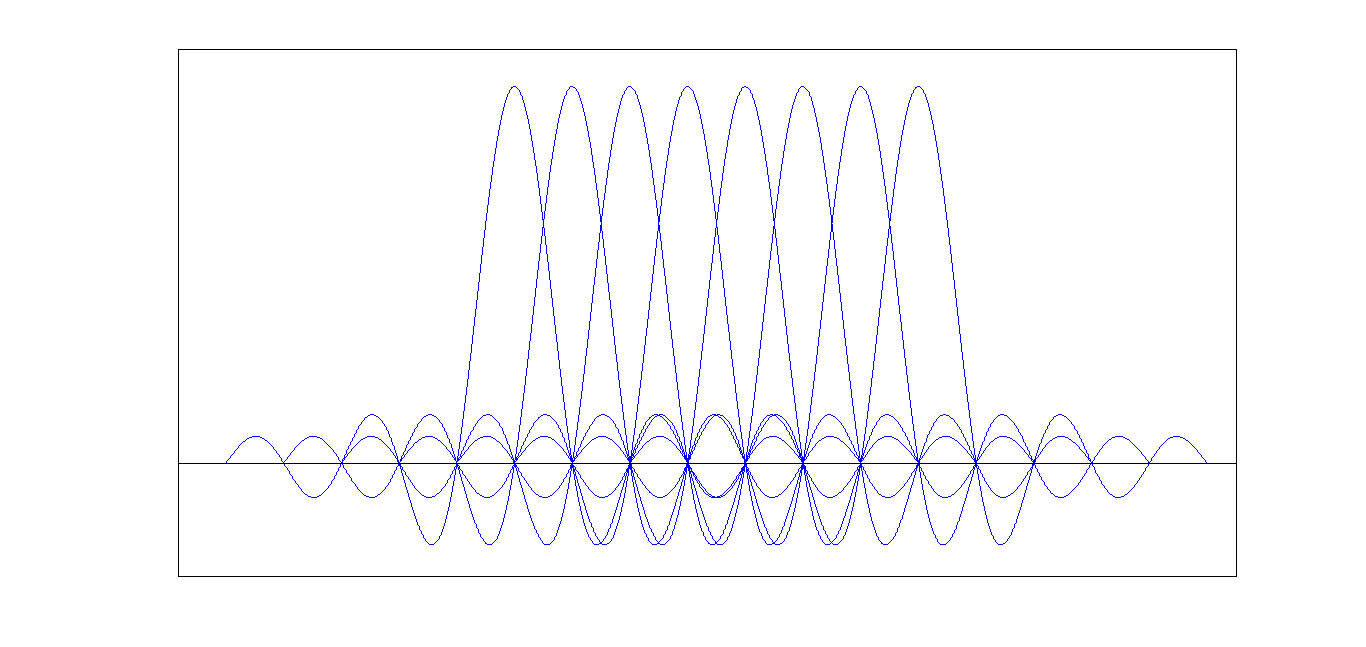
\includegraphics[angle = 0]{./figures/ofdm_subcarriers.png}}
% \end{minipage}
% \caption{OFDM sub-carriers scheme}
% \label{ofdm_carriers}
% \end{figure}

%The basis of the OFDM transmission is the sum of sub-carriers (which can be expressed by a complex exponential, or a \textit{frequency}
%in the complex plane) multiplied by the data symbols as expressed in equation (\ref{eq:OFDM_symbol_low}), where \textit{k} is the sub-carrier number.
The OFDM modulation scheme can be expressed as:

\begin{equation}
s_{k}(t-kT) =
%	\begin{cases}
	\sum\limits_{i=-N/2}^{N/2-1} x_{i,k} e^{j2\pi
	\left(\frac{i}{T}\right)(t-kT)}
%	\end{cases}
\label{eq:OFDM_symbol_low}
\end{equation}
where $x_{i,k}$ is the $i$th data symbol associated to the $k$th sub-carrier, and $T$ is the symbol period.

It is easy to recognize in (\ref{eq:OFDM_symbol_low}) an Inverse Discrete Fourier Transform. 
% (where the points in the frequency domain are translated to the time domain).\\
% Then, the OFDM modulator bank can be replaced by the computation of an IDFT and the demodulator bank by the computation of a
% DFT. It's possible to optize the implementation by using of efficient IDFT/DFT algorithms known as Fast Fourier Transform.\\
Assuming that $x_{i,k}$ is constant along the symbol period $T$ it is possible to use an Inverse Discrete Fourier Transform\slash Discrete Fourier Transform
(IDFT\slash DFT) blocks to modulate\slash demodulate the OFDM signal. This approach requires much less resources than using modulators\slash demodulators 
banks, moreover the IDFT\slash DFT might be computed by using the efficient Fast Fourier Transform (FFT) algorithm, 
which reduces the complexity of the algorithm from $\mathcal{O}(n^2)$ to $\mathcal{O}(n \, log n)$

The objective of this work is to obtain an FFT core, small enough to be included in a complete OFDM transceiver without consuming 
too much resources, but efficient and accurate enough to be useful in an Terrestrial Integrated Services Digital Broadcasting (ISDB-T) television system.

\section{Architecture selection}

There are several algorithms to calculate the FFT and each of them has some advantages and disadvantages. As we are trying to achieve a small
implementation, the radix-r algorithm is selected because of its particularity to reuse the same modules for all the steps involved in the FFT calculation \cite{Schaffer2_3}.
Radix-r algorithms are a variation of Cooley-Tukey algorithms \cite{MeyerRadix}, which factorizes the FFT length, $N$, in the form of $N = r^\nu$, such that the $N$-point FFT 
is decomposed in $\nu$ $r$-points sub-FFTs. This factorization reduces the complexity and leads to module reutilization as the sub-FFTs are all the same.
These are key advantages in order to reduce the footprint of the core.\\  
The main requirements for the implementation can be summarized in:

\begin{itemize}
  \item Run-time configurable FFT length, including at least 2K, 4K and 8K samples.
  \item $8,126,984$ sampling frequency guaranteed.
  \item Continuous input and output (not burst mode).
  \item Fixed point arithmethics.
  \item Run-time configurable and step-selectible scaling, with rounding and clipping options.
  \item Lower space consuption than other implementations like Xilinx FFT IPCore.
\end{itemize}

\subsection{Radix-r Algorithm}

This algorithm is based in the factorization of the FFT's length $N$ through the bidimentional mapping: 

\begin{equation}
n = N_2n_1 + n_2 \qquad 
	\begin{cases}
	0\leq n_1 \leq N_1 -1 \\
	0\leq n_2 \leq N_2 -1
	\end{cases}
\label{eq:CT_time_inedx}
\end{equation}

\begin{equation}
k = k_1 + N_1k_2 \qquad 
	\begin{cases}
	0\leq k_1 \leq N_1 -1 \\
	0\leq k_2 \leq N_2 -1
	\end{cases}
\label{eq:CT_freq_inedx}
\end{equation}
where $n$ is the time domain index, $k$ is the frequency domain index, and $N=N_1 \, N_2$.\\
The DFT and IDFT can be expressed as (\ref{eq:DTF}) and (\ref{eq:iDTF})

\begin{equation}
X[k] = \sum_{n=0}^{N-1}x[n]W_N^{kn}
\label{eq:DTF}
\end{equation}

\begin{equation}
x[n] = \frac{1}{N}\sum_{k=0}^{N-1}X[k]W_N^{-kn}
\label{eq:iDTF}
\end{equation}
where $W_N^{kn}=e^{\frac{-j2\pi kn}{N}}$ are known as \emph{twiddle factors}. 
Replacing (\ref{eq:CT_time_inedx}) and (\ref{eq:CT_freq_inedx}) in (\ref{eq:DTF}) and (\ref{eq:iDTF}) it is obtained:

\begin{equation}
X[k1,k2]=\sum_{n_2=0}^{N_2-1}
W_{N_2}^{n_2k_2}\left(W_{N}^{n_2k_1}\sum_{n_1=0}^{N_1-1}x[n_1,n_2]W_{N_1}^{n_1k_1}\right)
\label{eq:DFT_mod}
\end{equation}
The inner summation in (\ref{eq:DFT_mod}) is a $N_1$ points DFT multiplied by the factor $W_{N}^{n_2k_1}$. 
Taking $\tilde{x}[n2,k1]=W_{N}^{n_2k_1}\sum_{n_1=0}^{N_1-1}x[n_1,n_2]W_{N_1}^{n_1k_1}$
and replacing in (\ref{eq:DFT_mod}):

\begin{equation}
X[k1,k2]=\sum_{n_2=0}^{N_2-1}
W_{N_2}^{n_2k_2}\tilde{x}[n2,k1]
\label{eq:DFT_tilde}
\end{equation}
Equation (\ref{eq:DFT_tilde}) shows the $N_2$ points $\tilde{x}$ DFT. It demonstrates the power of the algorithm by replacing an $N$ point DFT
with two smaller sequential DFT. These sub-DFTs can be divided applying the described method in turn to reduce the original DFT to 
several sub-DFTs of smaller length and simpler to operate.

The value of $r$ affects the type and quantity of operations needed, as can
be seen in table \ref{table:FFT_oper}.

\begin{table}[h]
\centering
\caption{Operations needed by different values of \textit{r}  for an 8-point FFT}
\begin{tabular}{c c c c}
\textbf{r} & \textbf{Multiplications} & \textbf{Non trivial multiplications} &
\textbf{additions} \\ \hline 
$2$ & $2$ & $0$ & $2$ \\
$3$ & $3$ & $2$ & $6$ \\
$4$ & $4$ & $0$ & $8$ \\
$5$ & $6$ & $5$ & $17$ \\
$7$ & $9$ & $8$ & $36$ \\ \hline
\end{tabular}
\label{table:FFT_oper}
\end{table}
 
For $r=2$ and $r=4$ there aren't non trivial multiplications, so this are the values chosen for $r$.
A radix-r FFT has $log_rN$ stages and each stage has $N$ operations, giving the $\mathcal{O}(n \, log n)$ complexity. 
For $r=4$ more operations per stage are needed but there are
half the stages than for $r=2$. Then, both are implemented in order to compare them and bring the possibility to choose
depending on the requirements of the specific application.

Another advantage of this algorithm is the possibility of in-place memory using, where the results of an operation
is held in the memory position of the operands, so for an $N$ point DFT, an $N$ length memory is needed.

Radix-r algorithms limits the size of the FFT to powers of $r$, but it is not a trouble given that the available lengths are suitable for the proposed use.

\subsection{Implementation of the Radix-r architecture}

Fig. \ref{fig:r2_8} shows the simplified scheme for $8$ points radix-2 FFT.

Each node represents an addition and the arrows represents a multiplication by the value over it. 
Fig. \ref{fig:r2_8} shows the stage division of the algorithm, each of them performing a $2$ points DFT.
In general, for a $N$ points DFT $\frac{N}{2} \, \log_2(N)$ butterflies and $\frac{N}{2} \, (\log_2(N)-1)$ complex multipliers
are needed. There are different implementations for the radix algorithms which provides optimization in 
different aspects of the performance.

\begin{figure}[htb!]
        \centering
        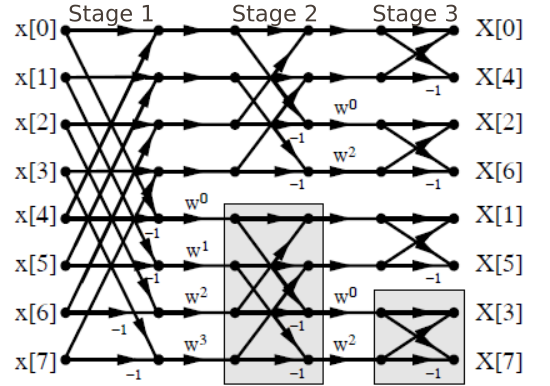
\includegraphics[width=6.5cm]{./figures/r2_8.png}
        \caption{8 points Radix-2 FFT algorithm representation}
        \label{fig:r2_8}
\end{figure}

Possible implementations are:

\begin{itemize}
  \item Parallel: All \textit{butterfly} and multipliers are implemented in similar scheme as 
  the one showed in Fig. \ref{fig:r2_8}.
  \item Unrolled: Single Delay Feedback (SDF) architecture \cite{torkelson}. Uses a \textit{butterfly} and a complex multiplier per stage.
  \item Iterative: Only one \textit{butterfly} and one complex multiplier, used sequentially
  by all the stages. Fig. \ref{fig:r2sBf} shows an $8$ points iterative radix-2 FFT scheme. 
\end{itemize}

\begin{figure}[htb!]
        \centering
        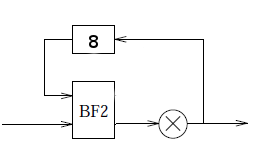
\includegraphics[width=6cm]{./figures/r2sBf.png}
        \caption{Iterative Radix-2 block diagram}
        \label{fig:r2sBf}
\end{figure}

Table \ref{table:radixcomp} shows the comparison of the characteristics of the three implementations described above.

\begin{table}[htb!]
\centering
\caption{Comparative between parallel, unrolled and iterative radix-r}
\begin{tabular}{l c c c}
\textbf{Characteristic} & \textbf{Parallel} & \textbf{Unrolled} &
\textbf{Iterative}\\
\hline 
\# \textit{butterfly} & $\frac{N}{\nu}*\log_\nu(N)$ & $\log_\nu(N)$ & $1$ \\
\# multipliers & $\frac{N}{\nu}*(\log_\nu(N)-1)$ & $log_\nu(N)-1$ & $1$ \\
Memory length & $0$ & $N-1$ & $N$ \\
Bus type & Parallel & Serial & Serial \\
\textit{throughput} & $N$ points per cycle & $1$ point per cycle & $1$ per $\log_\nu(N)$
cycles\\
\textit{pipeline} & Yes & Yes & No\\
\hline
\end{tabular}
\label{table:radixcomp}
\end{table}

In order to ensure the low space and low resource requirement, iterative implementation is chosen.

There are two differents approachs in radix algorithm implementations, decimation in time (DIT) and decimation in frequency (DIF). Both of them have the same 
complexity, so DIF is chosen because it is the most popular. 

\subsection{Twiddle factors multiplication}

Radix algorithms require the multiplication by twiddle factors. It is well known that multiplications in digital implementation are expensive  
in terms of space and time. Three methods were analyzed:
\begin{itemize}
  \item Cordic Algorithm
  \item Bajard, Kla and Muller (BKM) Algorithm
  \item Efficient complex multiplication
\end{itemize}

Twiddle factors have the form $W_N^{kn}=e^{\frac{-j2\pi kn}{N}}$. They represent a rotation in the complex axis. A well known and well proved 
algorithm for rotations is the cordic algorithm \cite{Volder}. It is based on successive approximations by micro-rotations until the desired angle is reached.
The main advantage of this algorithm is that it only uses additions (and subtractions) and shifts, both of them very cheap in terms
of resources. Also it can be pipelined, improving the speed of processing.\\

BKM algorithm resolves elemental equations using only additions and shifts \cite{BKM}. 
In comparison with Cordic Algorithm, BKM requires more storage and is more complex. In addition, its greater efficiency is obtained using 
redundant numeric system, which is not the case of the present work. Because of this reasons, BKM is discarded for this project.\\

In an iterative implementation, where only one multiplier is required, the difference between the cordic core and a complex multiplier is negligible.

For twiddle factors, the multiplication required is:
\begin{equation}
R+jI = (A+jB) \, (C+jD) = (A \, C-B \, D) + j(A\, D+B \, C)
\label{eq:prodcomp4}
\end{equation}
where $(C+jD)$ is the twiddle factor. A straight implementation would need four multipliers, but pre-calculating some of the factors and 
storing them in memory can reduce the implementation to three multiplications.
Pre-calculated factors are $C$, $(C+D)$ and $C-D$. Then, pre-calculated values 
are used to obtain $Z = C \, (A-B)$ and then:
\begin{equation}
R = (C-D) \, B + Z
\label{eq:prodcompR}
\end{equation}
\begin{equation}
I = (C+D) \, A - Z
\label{eq:prodcompI}
\end{equation}
 Taking into account that several FPGAs have DSP integrated modules, the implementation of multipliers could be very efficient.\\

Cordic and efficient complex multiplying are implemented as options because of the optimal resource utilization they features.

\subsection{Summary of the proposed implementation}

As it has been exposed in this section, the following architectures are implemented:

\begin{itemize}
  \item Radix-2 iterative architecture.
  \item Radix-4 iterative architecture.
  \item Cordic algorithm for twiddle factors multiplications, for radix-2 and radix-4.
  \item Efficient complex multiplier for twiddle factors multiplications, for radix-2 and radix-4, as an alternative to 
  cordic algorithm.
\end{itemize} 

\section{Radix-2}

In Fig. \ref{fig:r2_8} are shown the different stages of radix-2 FFT implementation.
On each clock cycle, one of two possible operations can be performed:

\begin{itemize}
  \item A point is stored in memory while another point is sent from memory to twiddle factor multiplier or to the core output.
  \item A butterfly operation between a core-input point or last-stage point and a memory-stored point. Two points results from the
  butterfly operation: one is stored in memory while the other is sent to the twiddle factor multiplier or to the output.  
\end{itemize}

%Figure (\ref{fig:radix2blocks}) provides a block diagram for radix-2 iterative implementation. There can be apreciated the main components 
The main components are an N-length memory, a butterfly, a complex multiplier an the control unit.

As it is needed to load a data and storage a data in every clock, then the memory is implemented as a dual-port RAM. 

In the butterfly the following operations are performed:
\begin{equation}
\begin{split}
c &= a+b \\
d &= a-b
\end{split}
\label{eq:butterf}
\end{equation} 
where $a$ and $b$ are complex inputs and $c$ and $d$ are complex outputs.

The control unit has to set the multiplexers according to the operation that is performed in that clock cycle, address the memory to the 
position where the actual operand is read or stored, and generate the twiddle factors for the multiplier.
Given that the core has $log_2(N)$ stages, the control unit has a stage-counter with length $log_2(log_2(N))$. Another counter, with a
length of $log_2(N)$ counts the number of points that have entered into the core by that moment. The control unit controls the whole core 
operation based on the stage and point number which are indicated by these counters.

\subsection{Integration}

Fig. \ref{fig:datapathmem} presents the integrated core. The control unit signals are showed as arrows to keep the graphic clear.
An additional register is placed before the multiplier because one result of a given stage is used in the following stage, so
it must be kept for one clock cycle. Another register is placed in the output in order to bring sequential synchronization 
with the circuit connected to the core.

An optional rounding/clipping unit is provided after the butterfly to give a method to deal with overflow. This can be turned on 
selectively for each stage in real time. 

\begin{figure}[htb!]
        \centering
        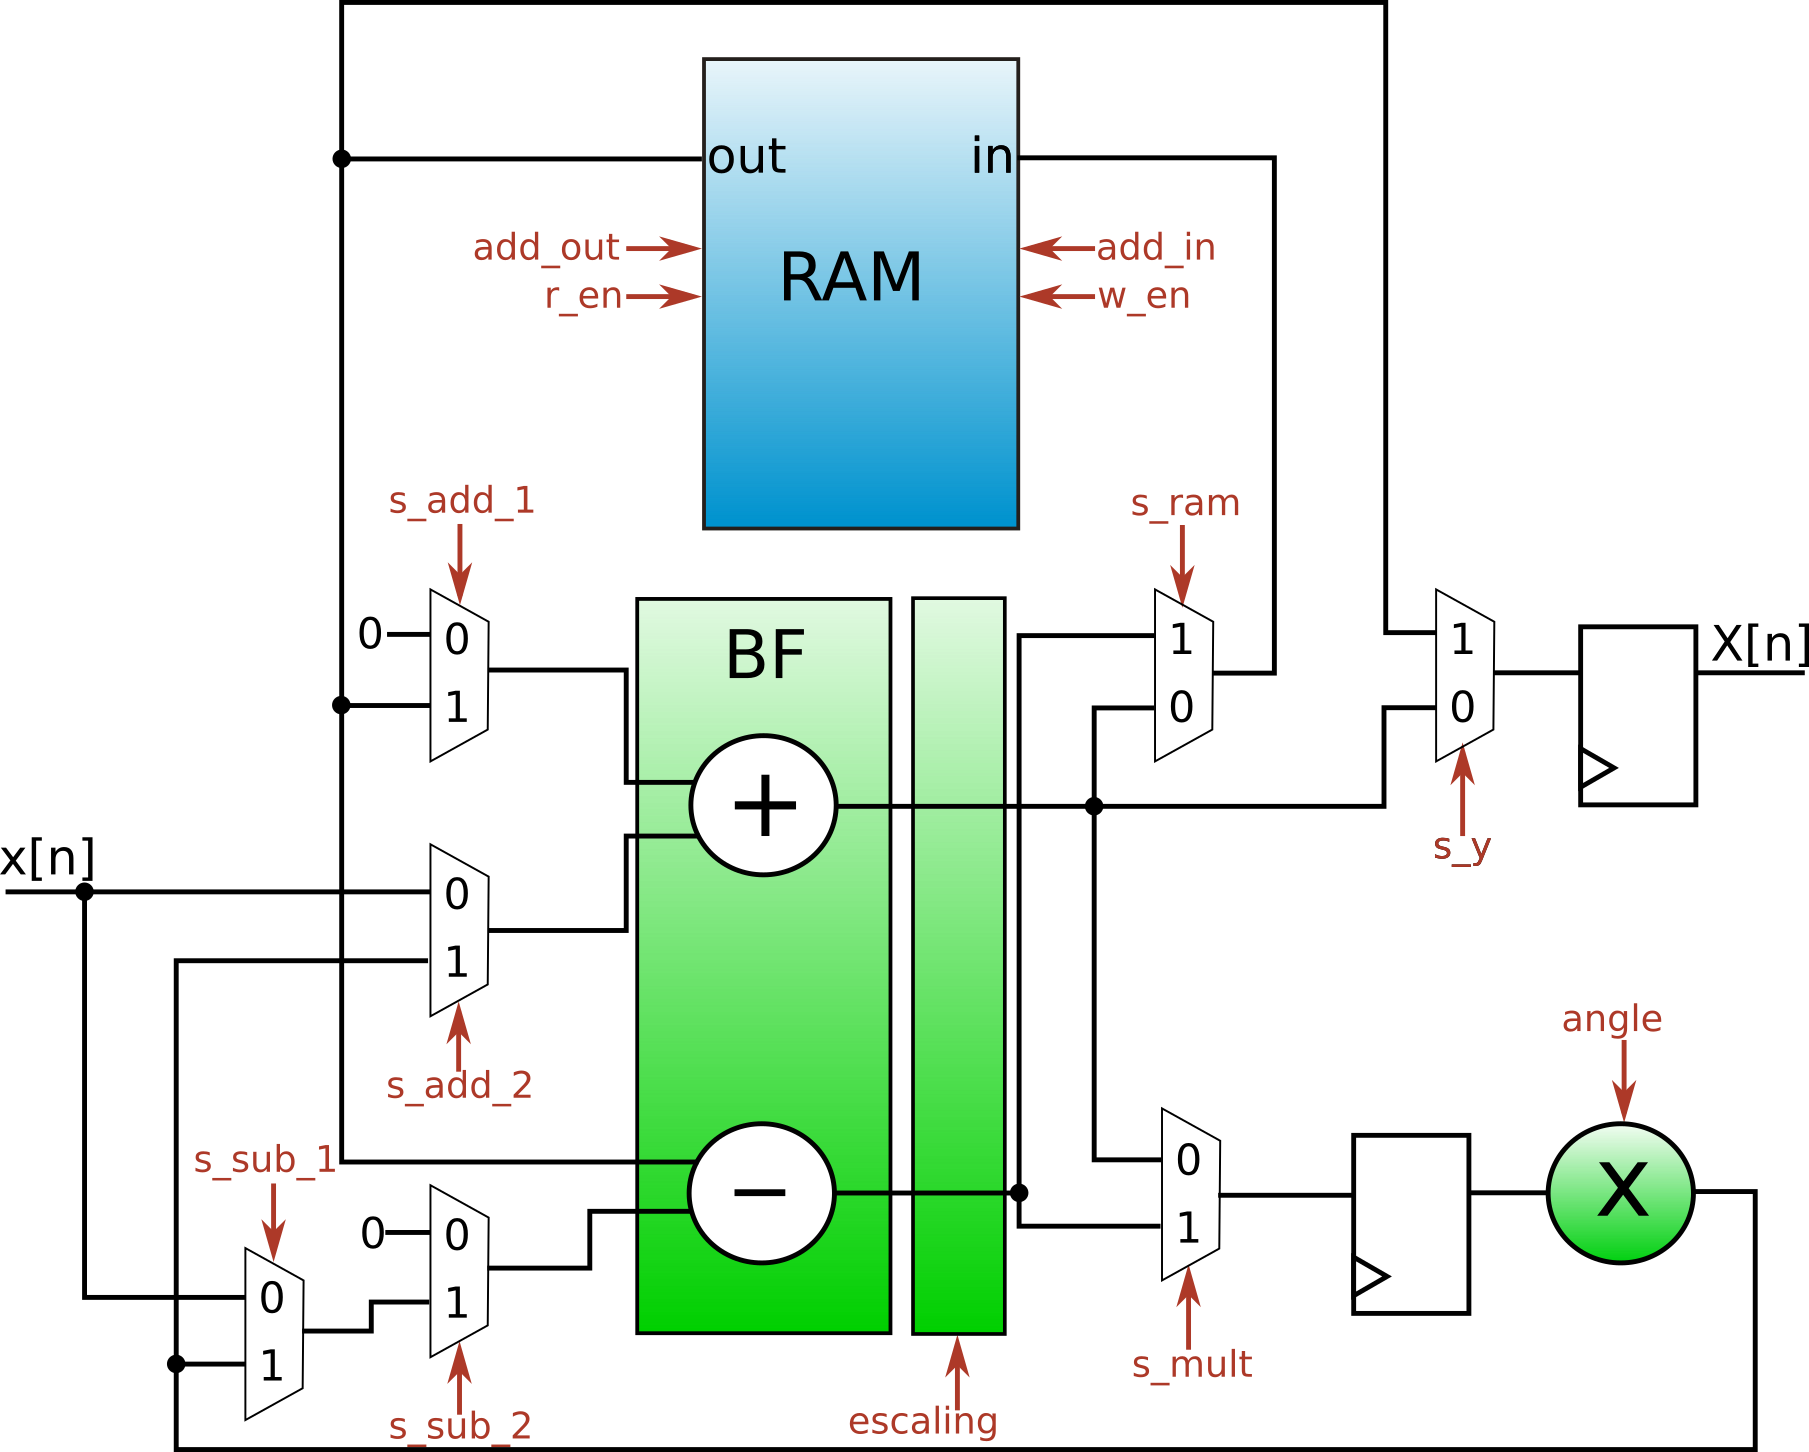
\includegraphics[width=9cm]{./figures/datapathMem.png}
        \caption{Iterative Radix-2 implementation diagram}
        \label{fig:datapathmem}
\end{figure}
 
\section{Radix-4}

The radix-4 algorithm divides a N-point DFT in $\nu$ 4-point DFT, so that $N = 4^\nu$.
The following expressions resumes the operations that the radix-4 has to process \cite{MeyerRadix}:

\begin{equation}
y_n = (x_n + x_{n+\frac{l}{4}} + x_{n+\frac{l}{2}} + x_{n+\frac{3l}{4}})
\label{eq:radix4_suby}
\end{equation}

\begin{equation}
z_n = ((x_n - x_{n+\frac{l}{2}}) -j (x_{n+\frac{l}{4}}
-x_{n+\frac{3l}{4}})) W_N^{k}
\label{eq:radix4_subz}
\end{equation}

\begin{equation}
g_n = ((x_n + x_{n+\frac{l}{2}}) - (x_{n+\frac{l}{4}}
+ x_{n+\frac{3l}{4}})) W_N^{2k}
\label{eq:radix4_subg}
\end{equation}

\begin{equation}
h_n = ((x_n - x_{n+\frac{l}{2}}) +j (x_{n+\frac{l}{4}} - x_{n+\frac{3l}{4}})) W_N^{3k}
\label{eq:radix4_subh}
\end{equation}
for $k = 0,1,\ldots,\frac{N}{4}-1$, where $l$ depends on the current processing stage.
Fig. \ref{fig:r4_diag} shows the operational scheme of a 16-points radix-4 algorithm.

\begin{figure}[htb!]
        \centering
        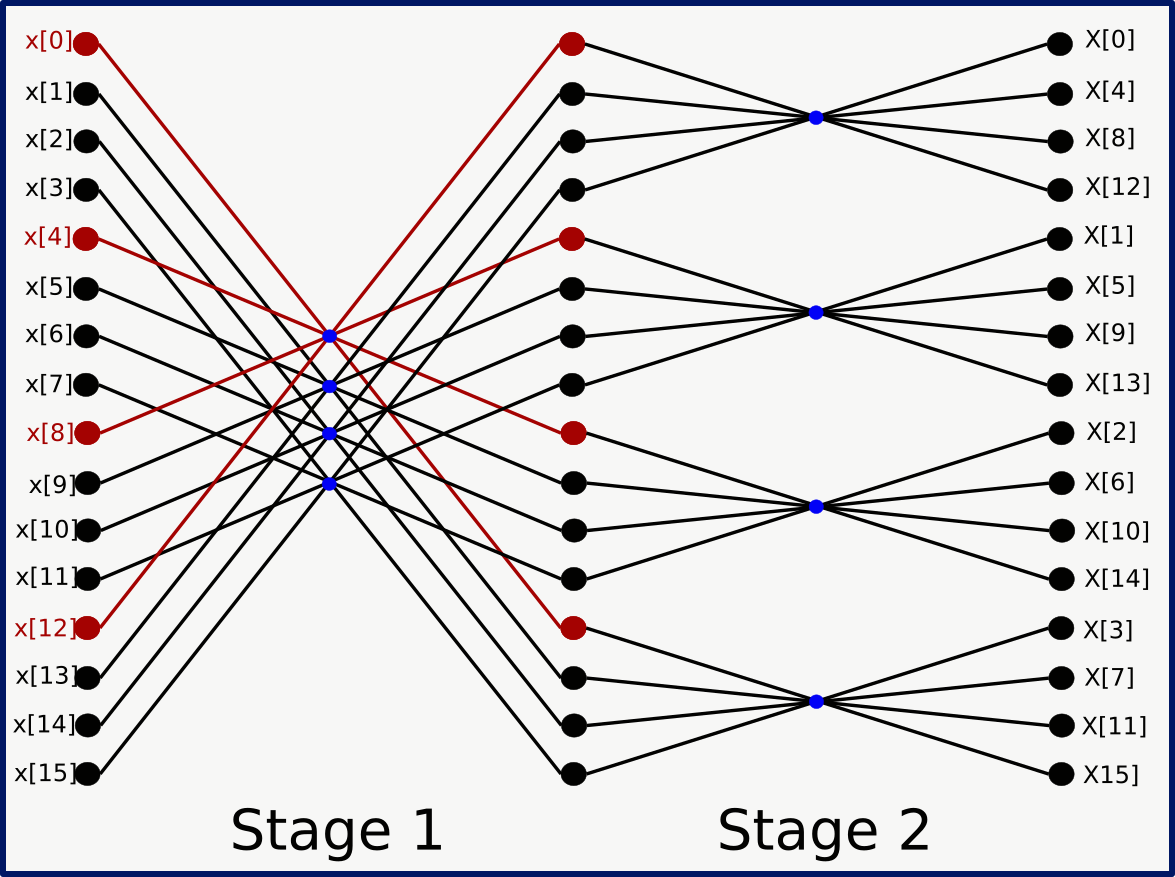
\includegraphics[width=6cm]{./figures/r4_16.png}
        \caption{16 points Radix-4 FFT algorithm representation}
        \label{fig:r4_diag}
\end{figure}

On each clock cycle, one out of four possible operations is performed:

\begin{itemize}
  \item A point is stored in a memory sub-block from the core input or the twiddle factor multiplier, while another point is sent 
  from the same memory sub-block to the multiplier or the output. For every sub-block, a different operation is considered.
  \item An arithmetic operation is performed with a point from the core input or the previous stage and 3 points from memory, each
  from a different memory sub-block. 
\end{itemize}

The main components are the memory, the arithmetic unit (called dragonfly), multiplier and the control unit, specially designed
for radix-4.

\subsection{Memory}

Each arithmetic operation needs four operands, one coming from the core input or the previous stage and another
three coming from the storage, so a 3-way in/3-way out memory is needed. In order to take advantage of memory blocks present 
in most FPGAs, a special memory is designed for this core. It is formed by three dual-port RAMs similar to the radix-2 memories, so
in each arithmetic operation, an operand of each memory sub-block can be read and stored simultaneously.\\
As the directions may not be successive, because in each clock cycle a different stage operation is performed, each sub block 
is divided in $\nu$ regions. The length of successive memory sub-blocks decreases as in the form $N/4$, $log_4(N/4)$, $Log_4(Log_4(N/4)) \ldots 1$. 
 
\subsection{Dragonfly}

The arithmetic unit calculates (\ref{eq:radix4_suby}) to (\ref{eq:radix4_subh}). In each stage two different 
types of operations can be performed: a four point arithmetic calculation or a memory data transfer.
In the last case, a point from a memory sub-block is transferred to the multiplier, while a point is stored in the next stage memory sub-block region.
The dragonfly unit includes an inner datapath which guides the data according to the operation in progress.
 
\subsection{Control unit}
 
As well as in radix-2, the control unit configures the datapath and generate the memory addresses and the twiddle factors for
the multiplier. As in radix-2, two counters are used: a $log_2(N)$ length points counter and a $log_2(log_4(N))$ length stage counter. 
%Determining which operation must be perform in a given clock cycle is done by evaluating the pair of the point counter's bits 
%refered by the value of the stage counter.\\
In order to determine which operation must be perform, two bits of the point counter are evaluated. These bits are selected using the stage
counter value. %The evaluated bits depends on the current stage, so they are choosen with the stage counter as showed in Fig. \ref{fig:r4_cont}.    
Memory addressing is done by mapping directly the point counter to the memory address. The sub-block region is selected with the 
stage counter because each sub-block is subdivided in regions for each stage. The read and write control signals are controlled according 
to the type of operation: in memory transfer operations only one sub-block is enabled while in arithmetical operations all three sub-blocks
are enabled to be read and written.

% \begin{figure}[htb!]
%         \centering
%         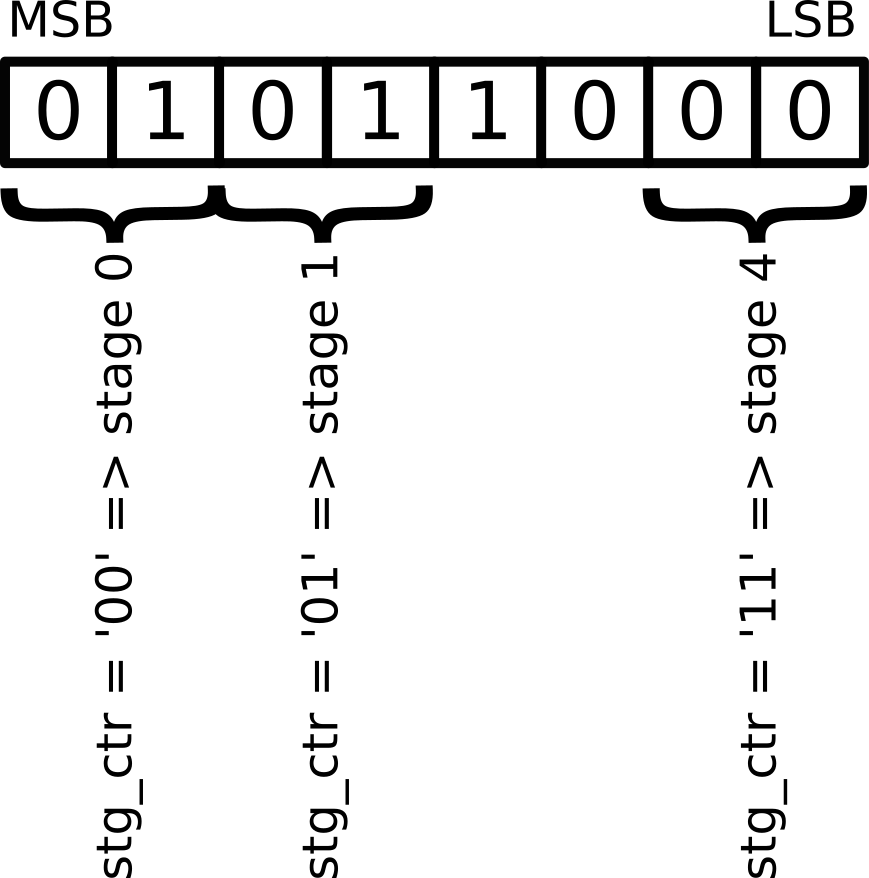
\includegraphics[width=4cm]{./figures/r4conts.png}
%         \caption{Point counter's bits to be evaluated in each clock}
%         \label{fig:r4_cont}
% \end{figure}

\subsection{Integration}

Fig. \ref{fig:datapathR4control} presents the iterative radix-4 core. As in radix-2 core, extra registers are added after the arithmetic unit and in 
the output. Also the rounding/clipping unit is added to the dragonfly to prevent overflow.  

\begin{figure}[htb!]
        \centering
        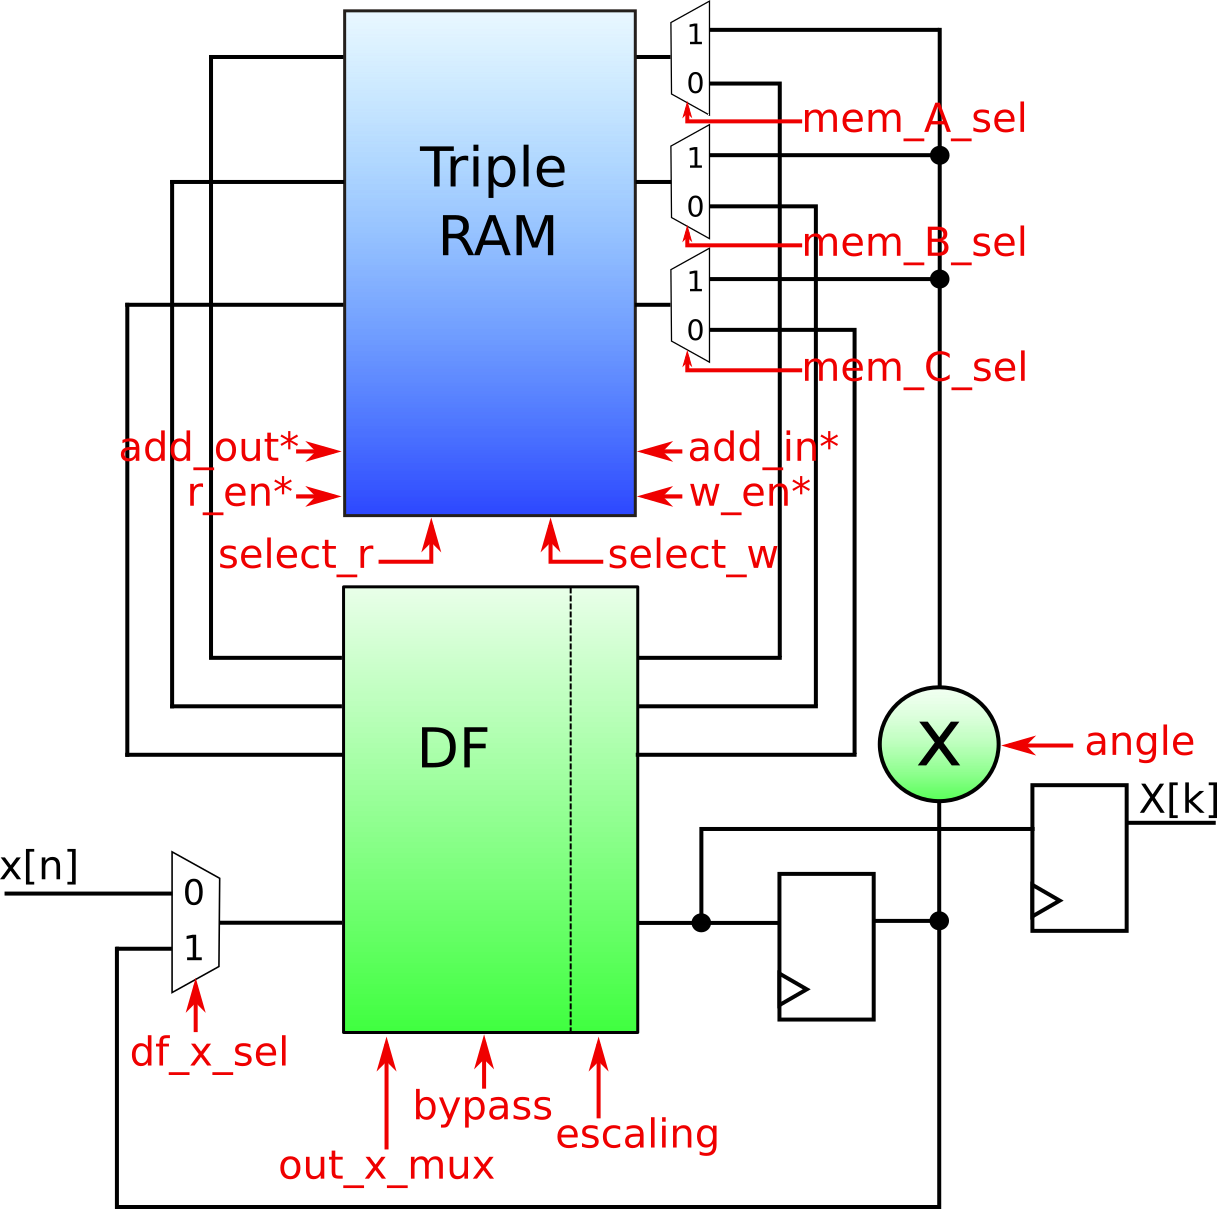
\includegraphics[width=7cm]{./figures/datapathR4control.png}
        \caption{Datapath with control signals}
        \label{fig:datapathR4control}
\end{figure} 
 
\section{Architecture Characterization}

Beside of the individual tests for every composing unit, a set of tests is performed over the entire architectures in order to verify and validate the design.
For a complete description of tests and results, refer to \cite{tesis}.

\subsection{Standard signals}
%First, a set of standard signals is applyed to the cores, and the result is compared to the expected result. The cores are
First, a set of basic tests are ran in the cores, and the results are compared to the expected results. The cores are
configured in IFFT mode.
The input and output signals are stated in table \ref{table:iout}:

\begin{table}[htb!]
\caption{Expected outputs for standard input signals}
\begin{tabular}{c c}
\textbf{Input} & \textbf{output}\\
\hline 
$\delta(0)$ & Constant signal \\
$\delta(6)$ & $\sin(\frac{2 \, \pi}{6})$ \\
$\sin(\frac{2 \, \pi}{6})$ & $\delta(6)$\\
\hline
\end{tabular}
\label{table:iout}
\end{table}
% \begin{itemize}
%   \item Delta in frequency component '0'. Expected a continuous signal.
%   \item Delta in frequency component 6. Expected six cycles of a sin.
%   \item Sin of period N/6. Expected a delta in time component 6.
% \end{itemize}

All the tests were passed correctly.

\subsection{Error measurement}

In order to measure the architecture error, the 64 bits floating point Matlab FFT is taken as a benchmark.

Two metrics are used for error measuring, $E_\infty$ and $E_2$:

\begin{equation}
E_\infty = \max\left(\frac{ X_o[n] - X_{dut}[n]}{X_o[n]}\right)
\label{eq:norma1}
\end{equation}

\begin{equation}
E_2 = \left\Vert\frac{X_o[n] - X_{dut}[n]}{X_o[n]}\right\Vert_2
\label{eq:norma2}
\end{equation}
where $X_o[n]$ is the Matlab FFT output and $X_{dut}[n]$ is the design under test output.

It is important to note that due to the quantization of the signals the architectures are non linear, so in order to obtain accurate 
error measurements, every test consists of $1024$ simulations with random vector inputs.
In each simulation, the result of the core computation is compared with Matlab results to obtain the error. After the $1024$ simulations, 
error values are averaged to obtain the final error values.
This is done for $12$ and $16$ bit implementations of radix-2 and radix-4 cores. This is because $12$ 
and $16$ bits are very commonly used word lengths in signal processing and OFDM communication systems. 
Also cordic and complex multiplier versions are tested, in order to compare their performance.
It is also measured the performance of a 16 bit integer C++ FFT, known as \emph{Kiss FFT} \cite{KISSFFT}.\\
%As an extra test bench, a widely used, 16 bit integer C++ FFT core is tested \cite{KISSFFT}. 
Test results are shown in table \ref{table:errorInf} and table \ref{table:error2}. It is clear that the performance of the cores is perfectly suitable for OFDM systems. 
Moreover, the cores meet the requirements to be used in signal processing as the error is under 1\%. For complex multiplier the error can be cutted down by increasing the word 
length of the factors stored in memory. For Cordic rotator, the error can be cutted down by adding rotation steps.\\

\begin{table}[htb!]
\caption{$E_\infty$ for 1024 simulations with random inputs}
\begin{tabular}{l c c c c}
 & \textbf{1024, 12 bits} & \textbf{1024, 16 bits} & \textbf{4096, 12 bits} & \textbf{4096, 16 bits}\\ \hline 
\textbf{Radix-2, Cordic} & $0.092$ & $0.006$ & $0.099$ & $0.008 $\\
\textbf{Radix-2, Mult.} & $0.232$ & $0.003$ & $0.340$ & $0.108$\\
\textbf{Radix-4, Cordic} & $0.077$ & $0.003$ & $0.074$ & $0.007$\\
\textbf{Radix-4, Mult.} & $0.224$ & $0.002$ & $0.334$ & $0.105$\\
\textbf{Kiss FFT} & $ $ & $0.017$ & $ $ & $0.035$\\\hline
\end{tabular}
\label{table:errorInf}
\end{table}

\begin{table}[htb!]
\caption{$E_2$ for 1024 simulations with random inputs}
\begin{tabular}{l c c c c }
 & \textbf{1024, 12 bits} & \textbf{1024, 16 bits} & \textbf{4096, 12 bits} & \textbf{4096, 16 bits}\\ \hline 
\textbf{Radix-2, Cordic} & $0.095$ & $0.007$ & $0.116$ & $0.053$\\
\textbf{Radix-2, Mult.} & $0.257$ & $0.004$ & $0.356$ & $0.131$\\
\textbf{Radix-4, Cordic} & $0.084$ & $0.002$ & $0.094$ & $0.027$\\
\textbf{Radix-4, Mult.} & $0.258$ & $0.003$ & $0.358$ & $0.126$\\ 
\textbf{Kiss FFT} & $ $ & $0.017$ & $ $ & $0.035$\\\hline
\end{tabular}
\label{table:error2}
\end{table}
 
% From tables \ref{table:errorInf} and \ref{table:error2} it is clear that the performance of the cores is perfectly suitable for OFDM systems. Moreover, 
% the cores meet the requirements to be used in signal processing as the error is under 1\%. For complex multiplier the error can be cutted down by increasing the word 
% length of the factors stored in memory. For Cordic rotator, the error can be cutted down by adding rotation steps.\\

\subsection{Total Harmonic Distortion}

In order to measure the THD of the architectures, sixteen test are performed. One for each architecture, radix-2 or radix-4, for all options 
described before: $12$ or $16$ bits, $1024$ or $4096$ points and cordic or complex multiplier for twiddle factors. Additionally, THD test is made 
over Kiss FFT to get a testbench \cite{KISSFFT}.\\
Each test runs consecutive simulations that use as input a tone in every input point each time. That way, a graphic can be made with 
the harmonic response to every frequency tone. Fig. \ref{fig:r2_thd_1024_cor} and Fig. \ref{fig:r4_thd_1024_cor} shows some of the 
results.\\

\begin{figure}[h!]
        \centering
        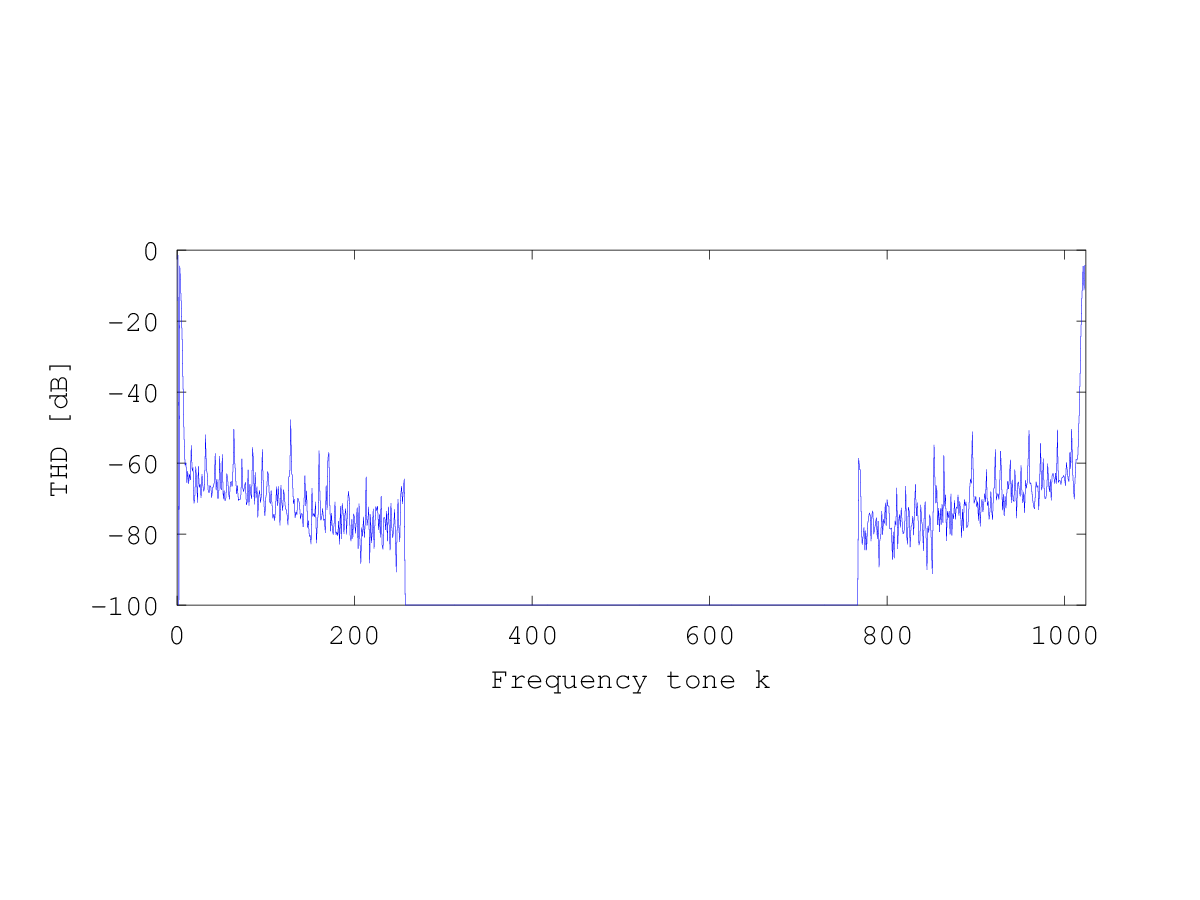
\includegraphics[width=10.7cm]{./figures/thd3.png}
        \caption{THD [dB] vs input tone frequency k for radix-2, Cordic, 12 bits.}
        \label{fig:r2_thd_1024_cor}
\end{figure}

\begin{figure}[h!]
        \centering
        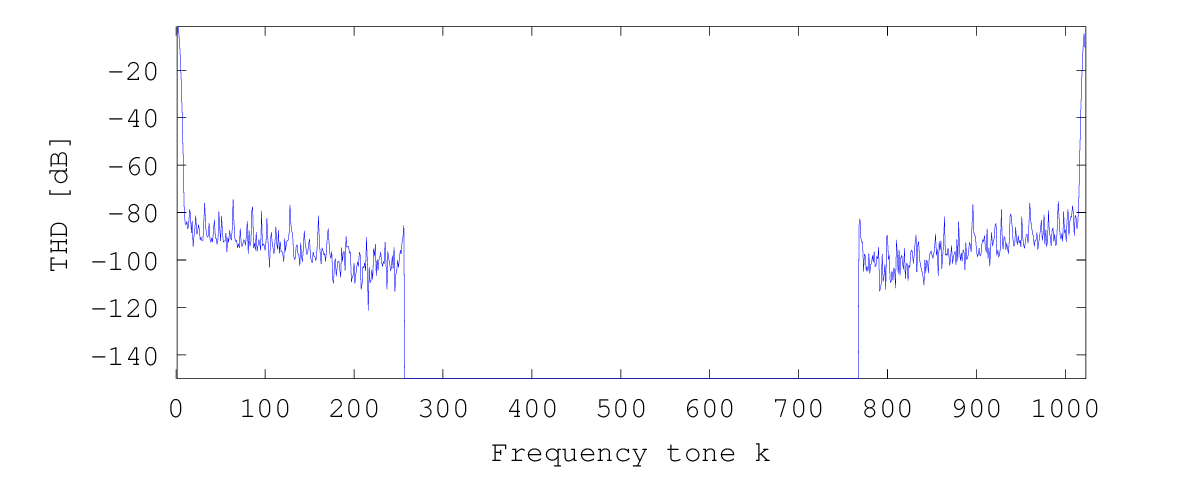
\includegraphics[width=10.7cm]{./figures/thd4_1.png}
        \caption{THD [dB] vs input tone frequency k for radix-4, Cordic, 16 bits.}
        \label{fig:r4_thd_1024_cor}
\end{figure}

\subsection{Test on Hardware}

For hardware validation, a Xilinx XC5XVL110 Virtex-5 FPGA is used. $1024$ points, $12$ bits iterative radix-2 and radix-4 are 
synthesized with Xilinx ISE v13.4 and routed into the FPGA along with a testbench circuit which provides PC connection via a UART port.

Standard signal and error tests, described above, are repeated on the hardware implementation obtaining same results as simulation tests, 
providing the successful on-hardware validation of the cores.

\subsection{Resource occupation}

The main requirement for the design is the low space/resource occupation. In order to validate this requirement accomplishment, $1024$ and $4096$, $16$ bits, iterative radix-2 and radix-4 architectures are 
synthesized. To have a comparative reference, a $16$ bits radix-2 sdf is implemented for $1024$ and $4096$ points.
Also, as a reference testbench, Xilinx's LogiCORE FFT v7.1 \cite{FFTXilinx} is synthesized.

Fig. \ref{fig:sizecomp1024} and Fig. \ref{fig:sizecomp4096} clearly shows that the designed cores are really small compared 
with another implementations, including a proprietary, device-optimized one like the LogiCORE FFT. Another important fact is that 
radix-4 and radix-2 needs approximately the same resource quantity, but radix-4 has double the throughput than radix-2.
\begin{figure}[htb!]
        \centering
        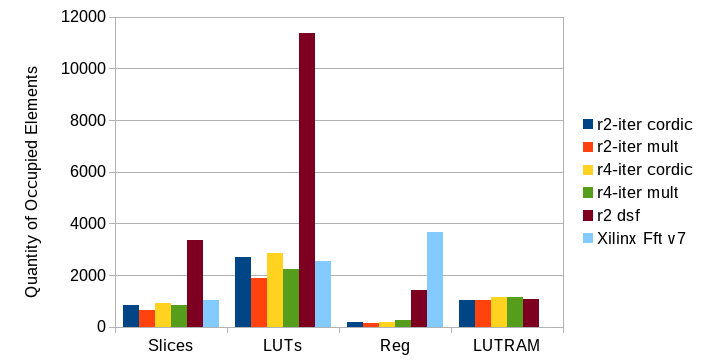
\includegraphics[width=9cm]{./figures/sizecomp1024.png}
        \caption{Size/resource comparison for 1024 points FFT}
        \label{fig:sizecomp1024}
\end{figure}

\begin{figure}[htb!]
        \centering
        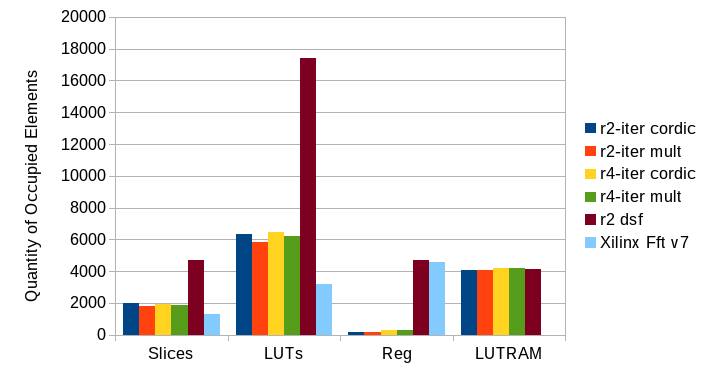
\includegraphics[width=9cm]{./figures/sizecomp4096.png}
        \caption{Size/resource comparison for 4096 points FFT}
        \label{fig:sizecomp4096}
\end{figure}  

\section{Conclusion}
This paper presented two iterative radix-r FFT computing cores, designed for OFDM
communication systems. Their main advantage is the extremely low space/resource consumption, which made them suitable for
integration in large systems without impacting in the resource distribution, in case of FPGA implementation, or space in case of
ASIC implementation. A complete description of the design and the verification and validation process has been presented.
 
The architectures were implemented in Verilog HDL code. Also there were developed several testing tools
comprising Matlab, C++ programs and Verilog testbenchs.

For future work, it can be considered to add a dithering system, in order to reduce the noise generated by the architectures, and 
to implement a pipelined cordic without modifying the global architecture timing, in order to improve the throughput. 



% trigger a \newpage just before the given reference
% number - used to balance the columns on the last page
% adjust value as needed - may need to be readjusted if
% the document is modified later
%\IEEEtriggeratref{8}
% The "triggered" command can be changed if desired:
%\IEEEtriggercmd{\enlargethispage{-5in}}

% references section

% can use a bibliography generated by BibTeX as a .bbl file
% BibTeX documentation can be easily obtained at:
% http://www.ctan.org/tex-archive/biblio/bibtex/contrib/doc/
% The IEEEtran BibTeX style support page is at:
% http://www.michaelshell.org/tex/ieeetran/bibtex/
%\bibliographystyle{IEEEtran}
% argument is your BibTeX string definitions and bibliography database(s)
%\bibliography{IEEEabrv,../bib/paper}
%
% <OR> manually copy in the resultant .bbl file
% set second argument of \begin to the number of references
% (used to reserve space for the reference number labels box)



\begin{thebibliography}{1}
\bibitem{Prasad2_1}                 Prasad, R. (2004), Orthogonal Frequency-Division Multiplexing. 
                                    In \textit{OFDM for Wireless Communications Systems} (p.p. 11-15), UK: Artech House.
\bibitem{Schaffer2_3}               Oppenheim, A., Shafer, R. (1999). The Discrete Fourier Transform. In
                                    \textit{Discrete-Time Signal Processing}, USA: Prentice Hall.
\bibitem{MeyerRadix}                J. W. Cooley and J. W. Tukey (1965) \textit{An algorithm for the machine calculation of complex Fourier series}, 
									Math. Comput., vol. 19, pp. 297-301.
\bibitem{torkelson}                 Shousheng H., Torkelson M. (1996). A New Approach to Pipeline FFT Processor.
                                    \textit{International Parallel Processing Symposium}
\bibitem{Volder}                    Volder, J. (1959). The Cordic computer technique. \textit{IRE. Trans. Elect. Comput.}
\bibitem{BKM}                       Bajard, J.C., Kla, S., Muller, J.C. (1994, Agosto). BKM: A New Hardware Algorithm for
                                    Complex Elementary Functions. \textit{IEEE Transaction on Computers 43}(8)
\bibitem{tesis}                     Cassagnes, A., Lutenberg, A., Giordano Zacchigna, F. (2016) ``Implementacion y analisis de algoritmos
                                    de calculo de Transformada Rapida de Fourier para su aplicacian en sistemas OFDM''
                                    http://laboratorios.fi.uba.ar/lse/tesis/LSE-FIUBA-Tesis-Grado-Andres-Cassagnes-2016.pdf
\bibitem{KISSFFT}                   https://sourceforge.net/projects/kissFFT/?source=navbar \textit{Kiss FFT is a very small, 
                                    reasonably efficient, mixed radix FFT library that can use either fixed or floating point data
                                    types.}
\bibitem{FFTXilinx}                 LogiCORE IP Fast Fourier Transform v7.1. (2011) Xilinx
\end{thebibliography}


\end{document}
